\chapter{Evaluation der Experimente}
\label{ch:versuche}

\blindtext{80}

\section{Abschnitt 1}
\label{sec:domain-stopwords}

\blindtext{30}
\begin{figure}[htbp]	
	\begin{minipage}{0.48\textwidth}
		\centering
		\caption{Wordcloud 1 - Rohdaten (reine \textit{Bag of Words})}
		\label{pic:wc-raw}
		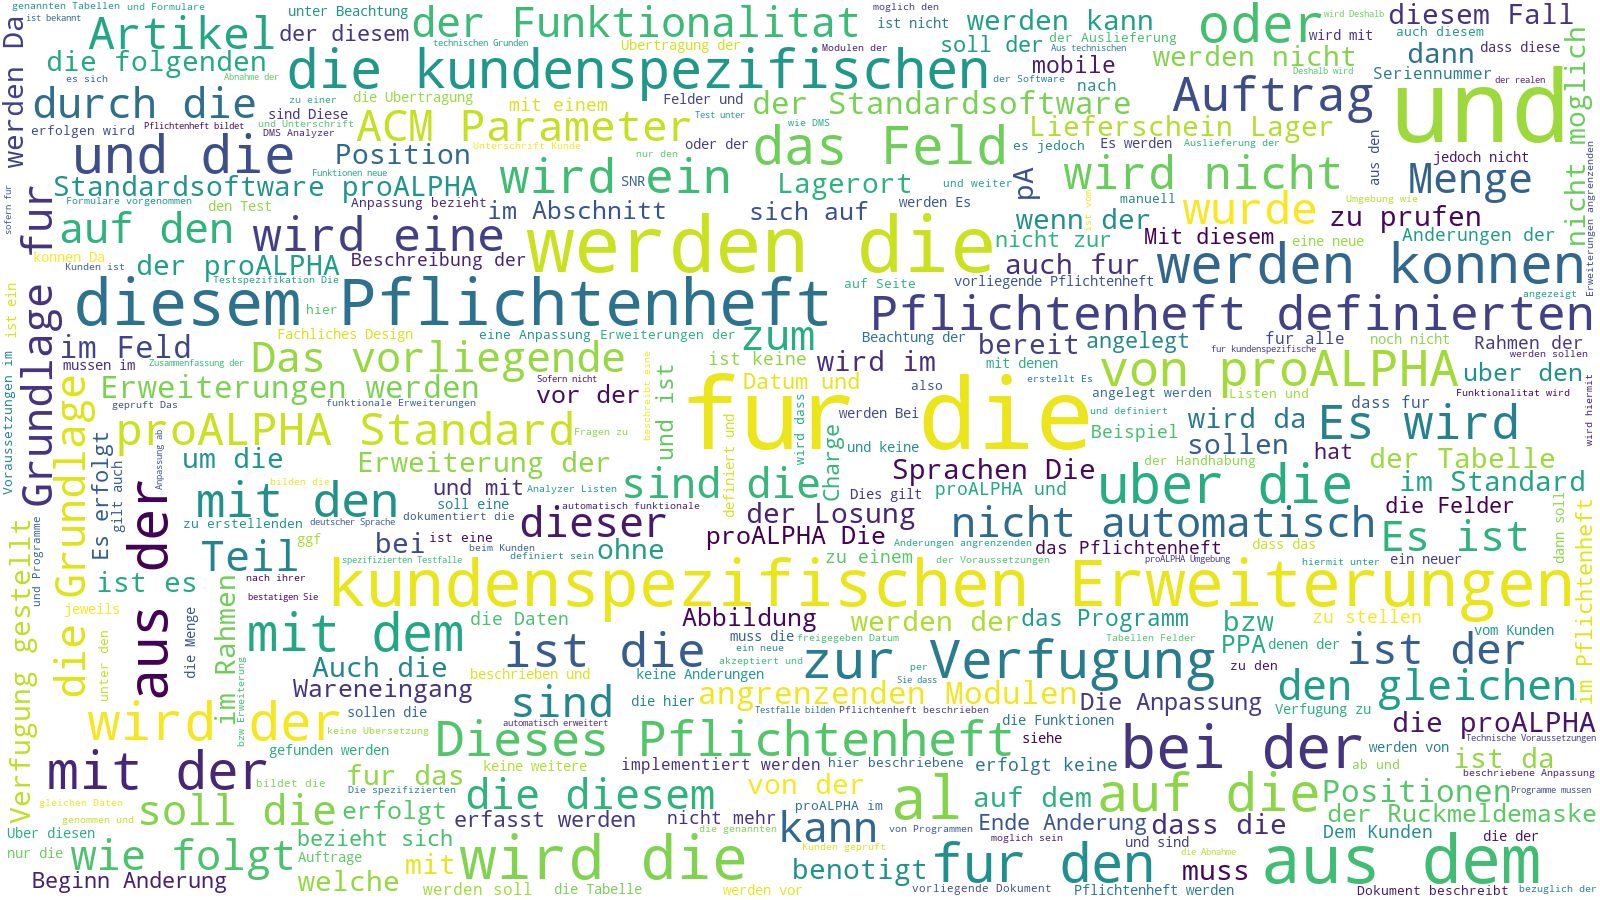
\includegraphics[width=6cm]{img/roh.png}
	\end{minipage}
	\hfill
	\begin{minipage}{0.48\textwidth}
		\centering
		\caption{Wordcloud 2 - nach Entfernung von deutschen \textit{stop-words}}
		\label{pic:wc-stops1}
		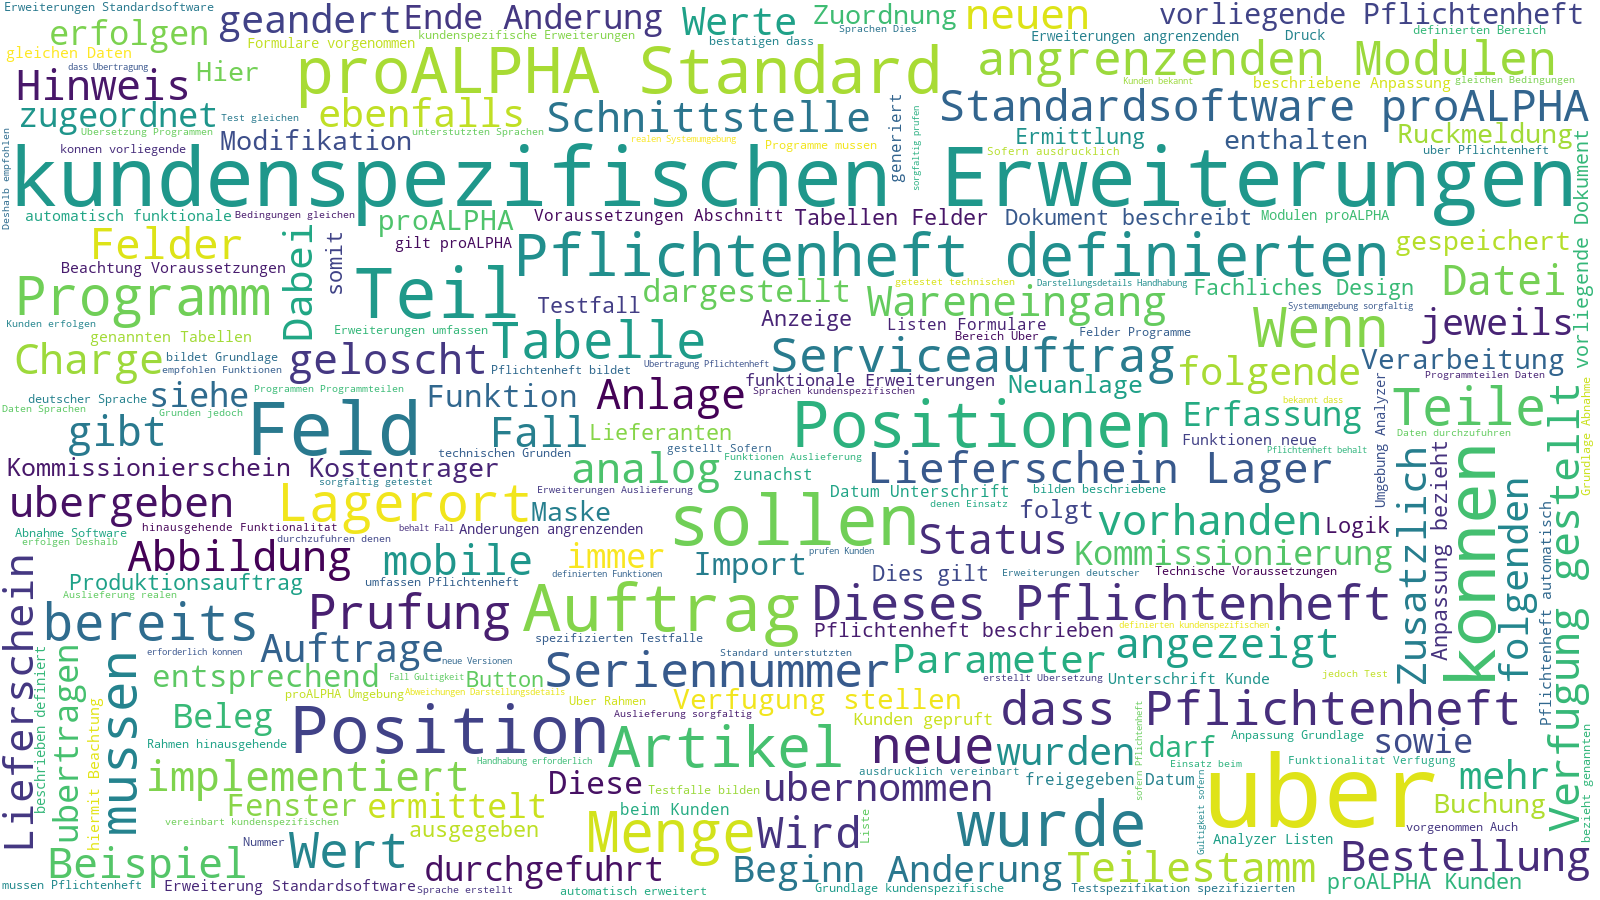
\includegraphics[width=6cm]{img/nurstop.png}		
	\end{minipage} 	
\end{figure}

\subsection{Unterabschnitt 1}

\begin{table}[htb]
	\centering
	\begin{tabular}{|c|c|c|c|} \hline
		Methode & \textit{Accuracy} & \textit{Precision} & \textit{Recall} \\ \hline
		hinge & 0.84541 & 0.83735 & 0.91285 \\
		log & 0.86956 & 0.83333 & 0.90452 \\
		modified\_huber & 0.86473 & 0.84278 & 0.91666 \\
		squared\_hinge & 0.69565 & 0.73129 & 0.78441 \\
		perceptron & \textbf{0.86956} & \textbf{0.85676} & \textbf{0.93871} \\ \hline
	\end{tabular}
	\caption{Durchschnittliche Performance für Durchlauf 1}
	\label{tab:methods-d1}
\end{table}

\blindtext{40}\\
\par
Hier verweise ich auf \ref{pic:wc-raw} und auf Abbildung \ref{pic:wc-stops1}\\
\par
\blindtext{60}


\pagebreak
\section{Fehlerbetrachtung}
\label{sec:fehler}

\blindtext{30}\par
\textcolor{red}{\textbf{Man sollte nicht außer Acht lassen, dass man das Bereits in der oen geziegten Tabelle \ref{tab:methods-d1} sieht.}}


